\documentclass[a4]{article}

\usepackage[left=3cm,right=3cm,top=2cm,bottom=2cm]{geometry} 

\usepackage[utf8]{inputenc}   % otra alternativa para los caracteres acentuados y la "ñ"
\usepackage[           spanish % para poder usar el español
                      ,es-tabla % para los captions de las tablas
                       ]{babel}   
\decimalpoint %para usar el punto decimal en vez de coma para los números con decimales

\usepackage[T1]{fontenc}
\usepackage{lmodern}

\usepackage{parskip}
\usepackage{xcolor}

\usepackage{caption}

\usepackage{enumerate} % paquete para poder personalizar fácilmente la apariencia de las listas enumerativas

\usepackage{graphicx} % figuras
\usepackage{subfigure} % subfiguras

\usepackage{amsfonts}
\usepackage{amsmath}

\definecolor{gris}{RGB}{220,220,220}
	
\usepackage{float} % para controlar la situación de los entornos flotantes

\restylefloat{figure}
\restylefloat{table} 

\newcommand{\HRule}{\rule{\linewidth}{0.5mm}}

\author{David Cabezas Berrido}
\date{\vspace{-5mm}}

\title{\huge Aprendizaje Automático: Práctica 1 \HRule\vspace{-4mm}}

\begin{document}
\maketitle
\tableofcontents

\newpage

\section{Ejercicio sobre la búsqueda iterativa de óptimos: Gradiente descendiente}

\subsection{Minimizar la función $E(u,v)$}

La función a minimizar es $E(u,v)=(ue^v-2ve^{-u})^2$, le aplicamos el algoritmo del gradiente 
descendente partiendo del punto $w=(1,1)$ con tasa de aprendizaje $\eta=0.1$.
La función es no negativa y sabemos que si encontramos un cero será un mínimo absoluto,
aceptamos un margen de error $\varepsilon=10^{-14}$ y nos interesa el punto en el que se alcanza
y las iteraciones necesarias para alcanzarlo. También he fijado un máximo de 100 iteraciones,
ya que no tengo asegurado encontrar un 0 y hay que añadir esa condición para asegurarnos
de que va a parar en algún momento.

He usado la librería \texttt{sympy} para el cálculo de las derivadas parciales en el programa.
También las he calculado analíticamente y el gradiente queda de este modo:

\begin{equation*}
\nabla E(u,v)=
\begin{pmatrix}
\frac{\partial E}{\partial u}(u,v) \vspace{2mm}\\
\frac{\partial E}{\partial v}(u,v)
\end{pmatrix}=
\begin{pmatrix}
    2(ue^v-2ve^{-u})(e^v+2ve^{-u}) \vspace{2mm}\\
    2(ue^v-2ve^{-u})(ue^v-2e^{-u})
    \end{pmatrix}
\end{equation*}

He ejecutado el algoritmo y, en sólo 10 iteraciones, he encontrado un valor por debajo de $\varepsilon$,
en el punto $w=(0.0447362903977822,0.0239587140991418)$.

\subsection{Estudio de la dependencia del \textbf{learning rate} ($\eta$)}

He utilizado el algoritmo del gradiente descendente para buscar un mínimo local de la función \\
$f(x,y)=(x-2)^2+2(y+2)^2+2\sin(2\pi x)\sin(2\pi y)$ partiendo desde el punto $(1,-1)$. Esta vez
realiza un número de iteraciones fijo (50 iteraciones), ya que desconozco los valores que puede
tomar la función y no puedo incorporar un criterio de parada como el de antes. Sí que podría incluir
como criterio la norma del gradiente, ya que ésta es casi 0 cuando estamos muy cerca del mínimo local.

El objetivo ésta vez es estudiar cómo afecta a la eficacia del algoritmo el valor escogido para la
tasa de aprendizaje $\eta$, para ello he ejecutado el algoritmo con dos valores diferentes de $\eta$
(0.01 y 0.1) y he medido el valor de la función en cada iteración, para estudiar la velocidad a la que
decrece o si se salta el mínimo y vuelve a crecer. En las siguientes gráficas se muestra cómo evoluciona
el valor de la función en cada iteración.

\begin{figure}[H]
    \centering    
    \subfigure[$\eta=0.01$]{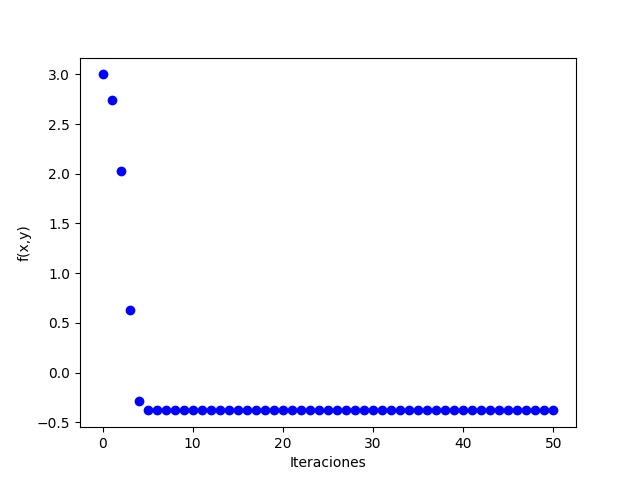
\includegraphics[width=77mm]{imgs/gd_0,01.png}}
    \subfigure[$\eta=0.1$]{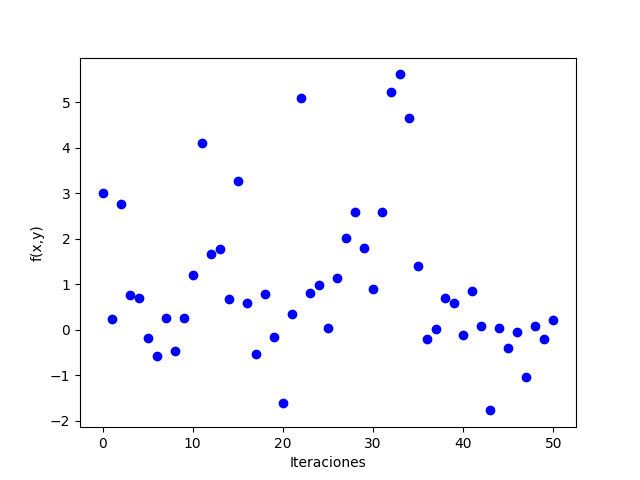
\includegraphics[width=77mm]{imgs/gd_0,1.png}}
    \caption{Comparación de la eficacia del algoritmo para dos valores de $\eta$.}
    \label{fig:comp-eta}
\end{figure}

Lo deseable es que la función decrezca lo más rápido posible. En el primer caso ($\eta=0.01$) se llega a un mínimo local
bastante rápido (se queda muy cerca en la quinta iteración) en el que la función toma el valor $-0.38124949743810027$,
en la segunda gráfica se aprecian valores de la función cercanos a -2, luego está claro que ese mínimo no es absoluto.

En cambio, la tasa de aprendizaje $\eta=0.1$ es demasiado alta y esto provoca que se salte el punto donde se alcanza el
mínimo local y el algoritmo no converja en el segundo caso. Es importante que la tasa de aprendizaje no sea demasiado alta
para evitar esto.

\subsection{Estudio de la dependencia del punto inicial escogido}

He ejecutado el algoritmo del gradiente descendiente para localizar mínimos locales en la función $f(x,y)$ partiendo
de distintas condiciones iniciales. Como no se especifica, he realizado 50 iteraciones y he fijado el valor $\eta=0.01$
como learning rate. He obtenido los siguientes resultados:

\begin{table}[H]
    \centering
    \begin{tabular}{|c|c|c|}
    \hline
                 & $(x,y)$ donde se alcanza el mínimo & $f(x,y)$                                        \\ \hline
    $(2.1,-2.1)$ &  $( 2.2438049693647883 ,  -2.2379258214861775 )$               & -1.8200785415471563 \\ \hline
    $(3,-3)$     &  $( 2.730935648248105 ,  -2.7132791261667033 )$              & -0.38124949743810005 \\ \hline
    $(1.5,1.5)$  & $( 1.7779244744891156 ,  1.032056872669696 )$                & 18.042078009957635  \\ \hline
    $(1,-1)$     &  $( 1.269064351751895 ,  -1.2867208738332965 )$              & -0.38124949743810027 \\ \hline
    \end{tabular}
\end{table}

\vspace{-5mm}

El algoritmo ha encontrado mínimos locales con valores muy diversos, lo que deja claro la dependencia del punto inicial.
Partiendo del punto $(1.5,1.5)$ he obtenido a una solución pésima, ya que ha quedado atrapado en un mínimo local con un
valor muy elevado. En cambio, partiendo del $(2.1,-2.1)$ he obtenido un
valor bastante cercano al mínimo absoluto, valor que no he obtenido con ninguna de las otras dos condiciones iniciales.

En este problema sé qué soluciones son buenas y cuales son malas porque he podido visualizar la función, pero en el caso
bastante común de que el espacio de funciones candidatas tenga dimensión mayor (haya que ajustar más de dos parámetros)
habría que minimizar una función de error que no se puede visualizar.

Por tanto, el mínimo absoluto de una función de
varias variables es muy difícil de encontrar con certeza, a no ser que la
función sea convexa. Así que la dificultad radica en que es difícil saber cuando
hemos elegido un punto inicial y un learning rate adecuados.


\section{Ejercicio sobre regresión lineal}

\subsection{Dígitos manuscritos}

Vamos a ajustar un modelo de regresión lineal a vectores de características
extraídos de imágenes de dígitos manuscritos (sólo de los dígitos 1, con
etiqueta -1 y 5, con etiqueta 1), concretamente el valor medio del nivel de
gris y simetría del número respecto al eje vertical. Lo haremos tanto por el 
algoritmo de la pseudoinversa como por el gradiente descendente estocástico.

\newpage

\subsubsection{Por pseudoinversa}
Con el algoritmo de la pseudoinversa, los pesos que he obtenido son
$w = [-1.11588016, -1.24859546, -0.49753165]$ y el plano solución el de esta
figura.

\vspace{-4mm}

\begin{figure}[H]
    \centering    
    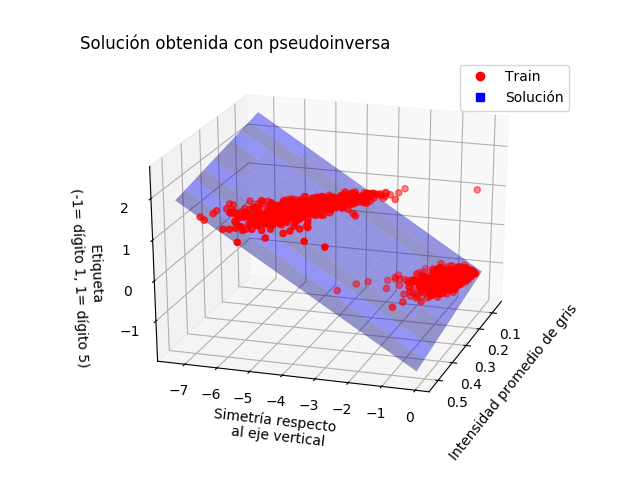
\includegraphics[width=100mm]{imgs/digitos-pinv.png}
    \caption{Plano obtenido con la pseudoinversa}
    \label{fig:digitos-pinv}
\end{figure}

\vspace{-5mm}

Bondad del ajuste: \quad
$E_{in}(w)=0.07918658628900388$ ,\qquad
$E_{out}(w)=0.13095383720052575$

\subsubsection{Por gradiente descendente estocástico}
Para el algoritmo del gradiente descendente estocástico, he usado el learning rate $\eta=0.001$, he fijado el tamaño de minibatch a 32 y he realizado 1000 iteraciones. Los pesos que he obtenido son
$w=[-1.23746596,-0.20592339, -0.44426966]$ y el plano
solución obtenido es el de esta figura. \vspace{-4mm}

\begin{figure}[H]
    \centering    
    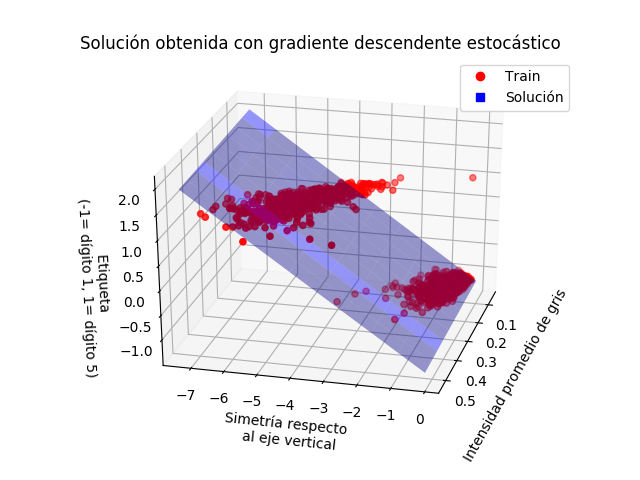
\includegraphics[width=100mm]{imgs/digitos-sgd.png}
    \caption{Plano obtenido con el gradiente descendente estocástico}
    \label{fig:digitos-sgd}
\end{figure}

\vspace{-5mm}

Bondad del ajuste: \quad
$E_{in}(w)=0.08341974836353012$ ,\qquad
$E_{out}(w)=0.13244457530997297$

Ligeramente peores debido a que es un método aproximado, pero bastante buenos.

\subsection{Ejercicio sobre la complejidad del modelo lineal}

Generamos una muestra de 1000 puntos uniformemente distribuidos en el intervalo
$\mathcal{X}=[-1,1]\times[-1,1]$, asignamos etiquetas
con la función $f(x_1,x_2)=\operatorname{sign}((x_1-0.2)^2+x_2^2-0.6)$ y
cambiamos el 10\% de las etiquetas para añadir ruido. La muestra queda de esta forma: \vspace{-4mm}

\begin{figure}[H]
    \centering    
    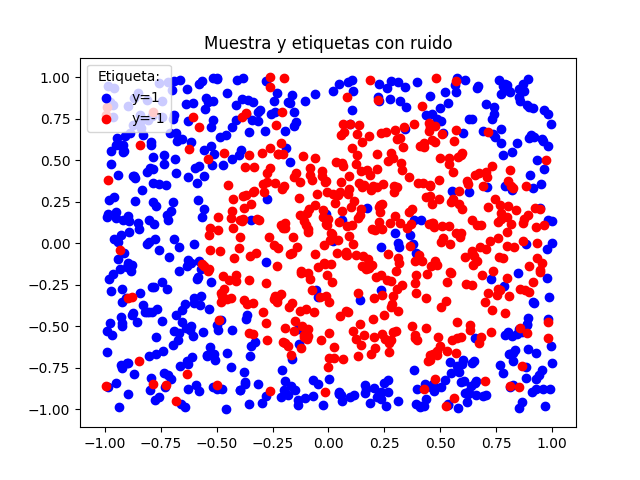
\includegraphics[width=100mm]{imgs/sample-noise.png}
    \caption{Muestra con ruido}
    \label{fig:sample-noise}
\end{figure} 

\vspace{-5mm}

Para los siguientes ajustes, he utilizado el algoritmo del gradiente descendente
estocástico con learning rate $\eta=0.001$, tamaño de minibatch 32 y 1000 iteraciones.

\subsubsection{Ajuste de un modelo de regresión con características lineales}
He ajustado un modelo de regresión lineal utilizando el vector de características
$(1,x_1,x_2)$, los pesos que he obtenido son $w=[0.04968622,-0.51886574,-0.0205383]$ y el plano solución es el siguiente. \vspace{-4mm}

\begin{figure}[H]
    \centering    
    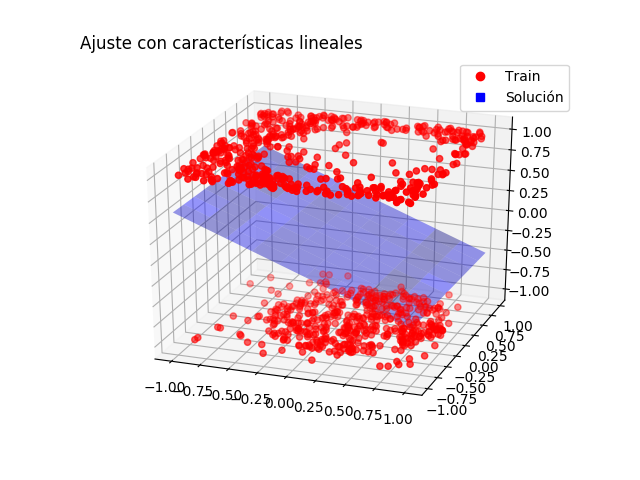
\includegraphics[width=100mm]{imgs/regress-lin.png}
    \caption{Plano obtenido utilizando características lineales}
    \label{fig:regress-lin}
\end{figure}

\vspace{-5mm}

He repetido el experimento 1000 veces y he obtenido los siguiente 
errores medios: \\
$E_{in}$ medio =  0.9240616367833707 ,\qquad
$E_{out}$ medio =  0.929279797769683

$E_{in}$ y $E_{out}$ están muy cercanos (lo que cabe esperar por la simplicidad del modelo).
No obstante, son muy altos, cosa que también esperaba tras observar la 
distribución, difícilmente iba a ser capaz de aproximar esa distribución con un plano.

\subsubsection{Ajuste de un modelo de regresión con características no lineales (cuadráticas)}

Esta vez, he ajustado un modelo de regresión lineal utilizando el vector de características
$(1,x_1,x_2,x_1 x_2,x_1^2,x_2^2)$, los pesos que he obtenido son
$w = [-0.83490846,-0.42438055,0.05310049,0.02361122,1.1982358,1.4037777]$
y la cuádrica solución es el siguiente. \vspace{-4mm}

\begin{figure}[H]
    \centering    
    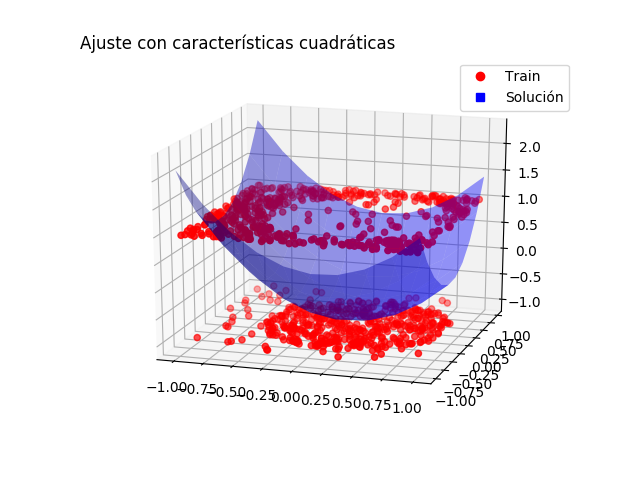
\includegraphics[width=100mm]{imgs/regress-nolin.png}
    \caption{Plano obtenido utilizando características lineales}
    \label{fig:regress-nolin}
\end{figure}

\vspace{-5mm}

He repetido el experimento 1000 veces y he obtenido los siguiente 
errores medios: \\
$E_{in}$ medio =  0.5643661965437399 , \qquad
$E_{out}$ medio =  0.5705303213340673

En esta ocasión, $E_{in}$ y $E_{out}$ no están significativamente más distantes
que en el modelo anterior a pesar del aumento de complejidad, y son bastante
menores. En la figura se aprecia que la cuádrica obtenida (un paraboloide elíptico) aproxima mucho mejor la distribución que el plano del caso anterior.

Por tanto, es obvio que \textbf{el modelo con características no lineales es más adecuado},
ya que obtiene mayor precisión en el ajuste. Consigue un $E_{out}$ menor, que
es el principal objetivo de la regresión.


\section{Ejercicio BONUS: Método de Newton y comparación con gradiente descendente}

He aplicado el Método de Newton para minimizar la función \\
$f(x,y)=(x-2)^2+2(y+2)^2+2\sin(2\pi x)\sin(2\pi y)$ de las secciones 1.2 y 1.3. Este método se usa para encontrar un cero en una función,
así que lo usamos para buscar un cero de la derivada.

Al igual que hice para el gradiente, he calculado con \texttt{sympy} la matriz
Hessiana de $f$. Sólo tengo que calcular 3 términos, ya que al ser $f$ de clase
2, $\frac{\partial^2 f}{\partial x\partial y}=\frac{\partial^2 f}{\partial y\partial x}$ (la Hessiana es simétrica).

A continuación están los resultados que he obtenido al realizar los experimentos
de las secciones 1.2 y 1.3, correspondientes al ejercicio 3 de Gradiente
Descendente. Hay una comparación con los resultados obtenidos usando el método de Newton y
el gradiente descendente, y la evolución del valor de $f(x,y)$ a medida que ambos algoritmos iteran.
Para el gradiente descendiente he fijado la tasa de aprendizaje $\eta=0.01$.
Ambos algoritmos realizan 20 iteraciones.

\begin{figure}[H]
    \centering    
    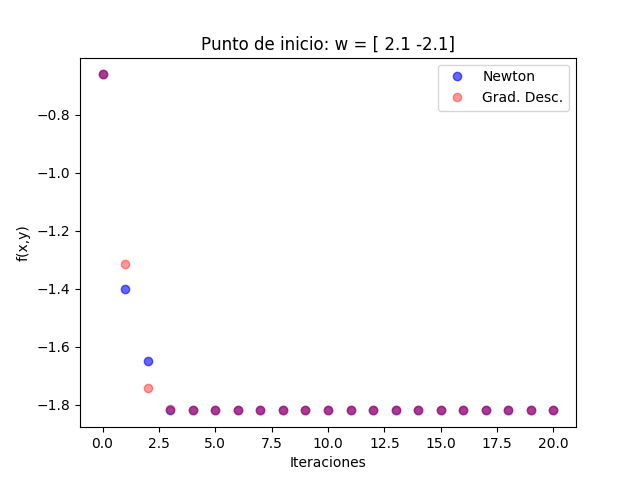
\includegraphics[width=100mm]{imgs/newton-grad_1.png}
    \caption{Newton frente a gradiente descendente, partiendo de $w=(2.1,-2.1)$}
    \label{fig:newton-grad_1}
\end{figure}

Punto de inicio: $w=(2.1 -2.1)$ \\
Solución y valor del método de Newton: \\
$(x,y) = ( 1.7561950306352117 ,  -1.7620741785138223 ) \qquad
f(x,y) =  -1.8200785415471563$ \\
Solución y valor del gradiente estocástico: \\
$(x,y) = ( 2.243804969364782 ,  -2.237925821486176 ) \quad
f(x,y) =  -1.8200785415471563$

\begin{figure}[H]
    \centering    
    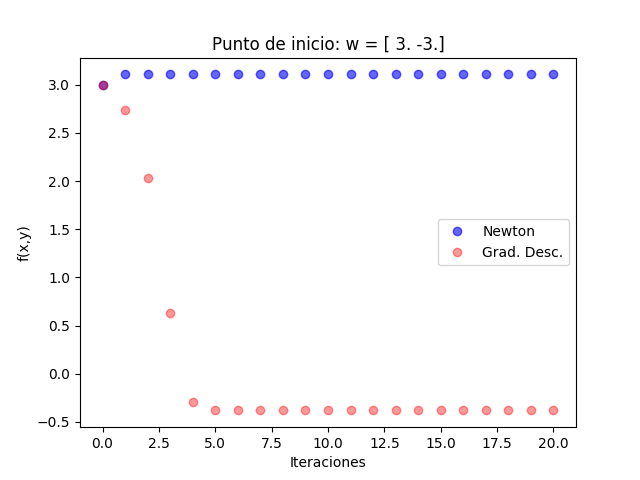
\includegraphics[width=100mm]{imgs/newton-grad_2.png}
    \caption{Newton frente a gradiente descendente, partiendo de $w=(3, -3)$}
    \label{fig:newton-grad_2}
\end{figure}

Punto de inicio: $w=(3, -3)$ \\
Solución y valor del método de Newton: \\
$(x,y) = ( 3.0539755549386394 ,  -3.028461459660191 ) \qquad
f(x,y) =  3.1079800610352017$ \\
Solución y valor del gradiente estocástico: \\
$(x,y) = ( 2.730935648250149 ,  -2.7132791261680187 ) \quad
f(x,y) =  -0.38124949743810027$

\begin{figure}[H]
    \centering    
    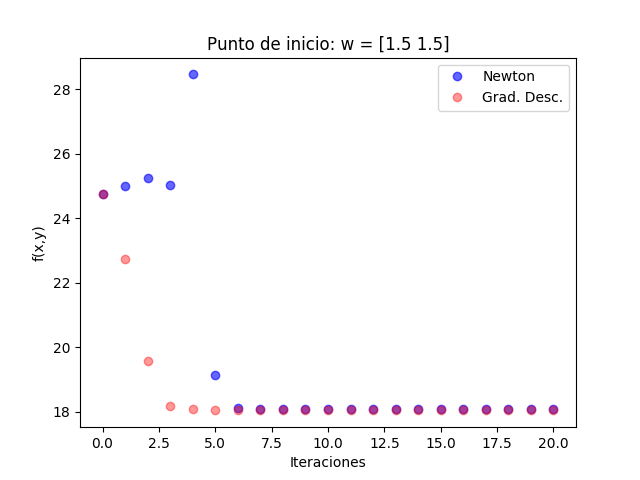
\includegraphics[width=100mm]{imgs/newton-grad_3.png}
    \caption{Newton frente a gradiente descendente, partiendo de $w=(1.5, 1.5)$}
    \label{fig:newton-grad_3}
\end{figure}

Punto de inicio: $w=(1.5, 1.5)$ \\
Solución y valor del método de Newton: \\
$(x,y) = ( 1.70483098300433 ,  0.9731715834776464 ) \qquad
f(x,y) =  18.08874203270784$ \\
Solución y valor del gradiente estocástico: \\
$(x,y) = ( 1.7730524579287212 ,  1.0365450542766357 ) \quad
f(x,y) =  18.042269888102044$

\begin{figure}[H]
    \centering    
    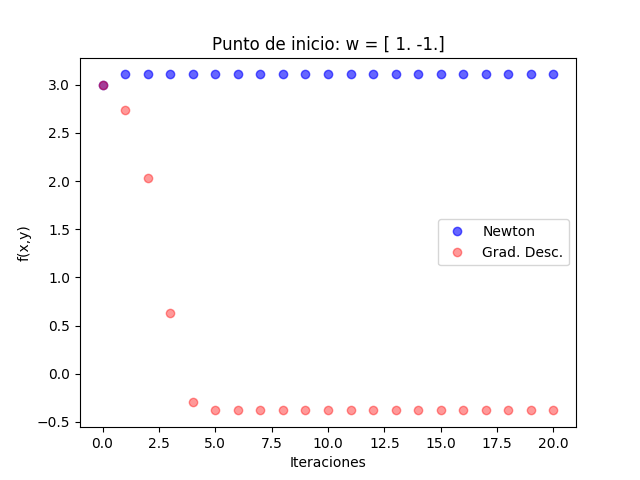
\includegraphics[width=100mm]{imgs/newton-grad_4.png}
    \caption{Newton frente a gradiente descendente, partiendo de $w=(1,-1)$}
    \label{fig:newton-grad_4}
\end{figure}

Punto de inicio: $w=(1 -1)$ \\
Solución y valor del método de Newton: \\
$(x,y) = ( 0.9460244450613605 ,  -0.9715385403398092 ) \qquad
f(x,y) =  3.107980061035202$ \\
Solución y valor del gradiente estocástico: \\
$(x,y) = ( 1.2690643517498512 ,  -1.2867208738319813 ) \quad
f(x,y) =  -0.38124949743810027$

\newpage

\textbf{\Large Valoración:} \\

El gradiente descendente, busca cero de la derivada, pero siempre avanza
hacia donde decrece la pendiente para así llegar a un mínimo local.
En cambio, el método de Newton se limita a buscar un cero de la derivada, independientemente de que sea un
mínimo local, máximo local o punto de silla.

Esto provoca que en algunas ocasiones, el método de Newton no proporcione un
mínimo local, sino otro punto crítico. Por eso no debe usarse como sustituto
del gradiente descendente, sino cuando sepamos que estamos muy cerca del mínimo.

Respecto a la precisión, ambos métodos han coseguido resultados
similares en los casos en los que el método de Newton no se ha
desviado hacia otro punto crítico. También es destacable
el hecho de que en ninguno de los cuatro experimentos, los
algoritmos hayan alcanzado la misma solución (el mismo $w$).

Aun así, el método de Newton sí tiene una ventaja, y es que no
hay que elegir un learning rate, por lo que no corremos
el riesgo de elegir uno inadecuado. Puede ser útil en
ocasiones en las que el gradiente descendente nos acerque a
un mínimo local pero no sea capaz de hallarlo con precisión.
\end{document}